% --------------------------------------------------------------------------
% the TASKS package
% 
%   Horizontal columned lists.
% 
% --------------------------------------------------------------------------
% Clemens Niederberger
% Web:    https://github.com/cgnieder/tasks/
% E-Mail: contact@mychemistry.eu
% --------------------------------------------------------------------------
% Copyright 2013-2014 Clemens Niederberger
% 
% This work may be distributed and/or modified under the
% conditions of the LaTeX Project Public License, either version 1.3
% of this license or (at your option) any later version.
% The latest version of this license is in
%   http://www.latex-project.org/lppl.txt
% and version 1.3 or later is part of all distributions of LaTeX
% version 2005/12/01 or later.
% 
% This work has the LPPL maintenance status `maintained'.
% 
% The Current Maintainer of this work is Clemens Niederberger.
% --------------------------------------------------------------------------
% If you have any ideas, questions, suggestions or bugs to report, please
% feel free to contact me.
% --------------------------------------------------------------------------
\documentclass[load-preamble+]{cnltx-doc}
\usepackage{tasks}

\setcnltx{
  package  = {tasks} ,
  authors  = Clemens Niederberger ,
  email    = {contact@mychemistry.eu} ,
  url      = {https://github.com/cgnieder/tasks/} ,
  info     = {create horizontal columned lists} ,
  add-cmds = {
    checkedchoicebox ,
    choicebox,
    NewTasks,
    settasks,
    startnewitemline ,
    task
  } ,
  add-silent-cmds = {
    choice, correct,
    DeclareInstance, DeclareTemplateInterface,
    leftthumbsup,
    sample, Sample
  }
}

\newpackagename\ExSheets{ExSheets}
\newpackagename\ExSheetslistings{ExSheets-listings}
\newpackagename\cntformats{cntformats}
\newpackagename\Tasks{tasks}

% ----------------------------------------------------------------------------
% other packages, bibliography, index
\usepackage{xcoffins,tikz,wasysym,enumitem,booktabs,siunitx}
\usepackage[accsupp]{acro}
\DeclareAcronym{id}{
  short     = id ,
  long      = Identifier ,
  format    = \scshape ,
  pdfstring = ID ,
  accsupp   = ID
}

\usepackage{filecontents}
\usepackage{csquotes}



% ----------------------------------------------------------------------------
% example definitions that have to be done in the preamble:
\usepackage{exsheets}
\usepackage{dingbat}
\NewTasks[style=multiplechoice]{multiplechoice}[\choice](3)
\newcommand*\correct{\PrintSolutionsTF{\checkedchoicebox}{\choicebox}}


\newcommand*\sample{This is some sample text we will use to create a somewhat
  longer text spanning a few lines.}
\newcommand*\Sample{\sample\ \sample\par\sample}

\begin{document}

\section{Motivation}
Originally \Tasks\ has been an integral part of the
\ExSheets\changedversion{0.7} package.  However, users told me that it indeed
could be useful to have it as a stand-alone package not having to load the
whole \ExSheets\ beast just for having the \env{tasks} environment available.
Since I agree with this the environment has been extracted into a package if
its own, \Tasks.  Since then \Tasks{} has been distributed as a package of its
own but as part of the \ExSheets{} bundle\changedversion{0.10}.  With v0.10 I
decided to make it a completely independent package.  So the relation to
\ExSheets{} only is a historical one.

The reason for the \env{tasks} environment is an unwritten agreement in German
maths textbooks (exspecially in (junior) high school textbooks) to organize
exercises in columns counting horizontally rather than vertically.  That is
what \code{tasks} primarily is for. If you don't need this feature you're
better off using traditional \LaTeX{} lists and the \pkg{enumitem} package for
customization.

\section{License and Requirements}\label{sec:license}
\license

\Tasks\ requires the \bnd{l3kernel}~\cite{bnd:l3kernel} bundle,
\needpackage{xparse}, \pkg{xtemplate} and \needpackage{l3keys2e} which are
part of the \bnd{l3packages}~\cite{bnd:l3packages} bundle,
\pkg{epic}~\cite{pkg:epic}, \pkg{cntformats}~\cite{pkg:cntformats}, and
\pkg{environ}~\cite{pkg:environ}.


\section{How it works}
\subsection{The Basics}
The \env{tasks} environment is similar to a list like \env{enumerate} but not
the same.  Here are some of the differences:
\begin{itemize}
  \item A first difference: there is no pagebreak possible inside an item but
    only between items.
  \item A second difference: the enumeration default is a), b), c) \ldots
  \item A third difference: the body of the \env{tasks} environment is split
    at \emph{every} occurrence of the item separator.  For this reason the
    default separator is not \cs*{item} but \cs{task} so it is unique to this
    environment only.  This directly leads to\ldots
  \item \ldots{} a fourth difference: the \env{tasks} environment cannot be
    nested.  You can, however, use an \env*{itemize} environment or another
    \enquote{real} list in it.
  \item A fifth difference: verbatim material cannot be used in it.  You'll
    have to use \cs*{string}, \cs*{texttt} or \cs*{detokenize}.  If this
    won't suffice then don't use \env{tasks}.
%  \item A sixth difference: %footnotes
\end{itemize}

\begin{environments}
  \environment{tasks}[\oarg{options}\darg{num of columns}]
    List like environment where the single items are introduced with
    \cs{task}.
\end{environments}
Let's see an example:
\begin{example}
  % \Sample is defined to contain some sample text:
  % \def\sample{This is some sample text we will use to create a somewhat
  %   longer text spanning a few lines.}
  % \def\Sample{\sample\ \sample\par\sample}
  Some text before the list.
  \begin{tasks}
    \task \Sample
    \task \Sample
    \task \Sample
  \end{tasks}
  And also some text after it.
\end{example}

The environment takes the optional argument \darg{num of columns} with which
the number of columns used by the environment is specified.
\begin{example}
  \begin{tasks}(2)
    \task \Sample
    \task \sample\ \sample
    \task \sample
    \task \Sample
    \task \sample\par\sample
  \end{tasks}
\end{example}

\subsection{Items Spanning More Than One Column}
Sometimes it may come in handy if an item is allowed to span more than one
column.  \Tasks\sinceversion{0.10} supports items using the remaining space by
adding an optional\label{optional-star} star to \cs{task}:
\begin{example}
  \begin{tasks}(3)
    \task \sample
    \task* \sample
    \task* \sample
    \task \sample
    \task \sample
  \end{tasks}
\end{example}

\Tasks\sinceversion{0.10} also supports items that span \emph{all} columns in
any case by adding an optional bang\label{optional-bang} to \cs{task}.
\begin{example}
  \begin{tasks}(3)
    \task \sample
    \task! \sample
    \task! \sample
    \task \sample
    \task \sample
  \end{tasks}
\end{example}

The optional star has itself an optional argument with parentheses where you
can specify the number of columns the item is supposed to span:\label{debug}
\begin{example}
  \settasks{debug}
  \begin{tasks}(4)
    \task the first
    \task the second
    \task the third
    \task the fourth
    \task*(3) the fifth item is way too long for this and needs three columns
    \task the sixth
    \task the seventh
    \task*(2) the eighth item is way too long for this and needs two columns
    \task the nineth
    \task the tenth
  \end{tasks}
\end{example}
If there are not enough columns left (say two columns but you said
\cs{task}\sarg\Darg{3}) the argument is ignored and the maximum number of
remaining columns is used (two in case of our example).

Both optional star and optional bang can be combined with the optional
argument for a custom label:
\begin{example}
  \begin{tasks}(3)
    \task \sample
    \task* \sample
    \task*[(x)] \sample
    \task \sample
    \task \sample
  \end{tasks}
\end{example}

Forcing a new item line manually is also possible\sinceversion{0.9} using the
following command:
\begin{commands}
  \command{startnewitemline}
    Introduce a new line in a \env{tasks} environment.
\end{commands}
\begin{example}
  \begin{tasks}(4)
    \task the first
    \task the second
    \task the third
    \task the fourth
    \task \rlap{the fifth item is way too long for this so we start a new row}
      \startnewitemline 
    \task the sixth
    \task the seventh
    \task \rlap{the eighth item also is too long} \startnewitemline
    \task the nineth
    \task the tenth
  \end{tasks}
\end{example}

While this works it also needs a bit of care since the wisth of the items
doesn't change which means in order to use the full width you'd have to use
trickery like \cs*{rlap} which then means the danger of the item text sticking
into the margin\ldots

\section{Available Options}\label{sec:tasks:options}

The \Tasks{} package does not have any package options\changedversion{0.10}.

The environment \env{tasks} has a number of options, though, namely the
following ones that can be set using a setup command:
\begin{commands}
  \command{settasks}[\marg{options}]
    Setup command for \Tasks.
\end{commands}
\begin{options}
  \keyval{style}{instance}\Default
     Choose the instance to be used.  Read more on this in
     section~\ref{sec:tasks}.
  \keyval{counter-format}{counter specs}\Default
    \sinceversion{0.9}Sets a custom label.  The letters \code{tsk} are
    replaced with the task-counter.  An optional argument directly following
    these letters specifies the counter format: \code{1}: \cs*{arabic},
    \code{a}: \cs*{alph}, \code{A}: \cs*{Alph}, \code{r}: \cs*{roman} and
    \code{R}: \cs*{Roman}.
  \keyval{label-format}{code}\Default
    \changedversion{0.9}Can be used to apply a formatting like, \eg,
    \cs*{bfseries} to the labels.
  \keyval{label}{code}\Default
    \changedversion{0.9}Overwrite the automatic label to a custom one.
  \keyval{label-width}{dim}\Default{1em}
    Sets the width of the item labels.
  \keyval{label-offset}{dim}\Default{.3333em}
    \sinceversion{0.7}Sets the offset, \ie, the distance between label and
    item.
  \keyval{item-indent}{dim}\Default{2.5em}
    \sinceversion{0.9a}The indent of an item, \ie, the horizontal space
    available for both label and label-offset.  If
    \[
      \text{\code{indent}} =
      \text{\code{label-width}} + \text{\code{label=offset}}
    \]
    the label will align with the textblock above (if
    \keyis{label-align}{left} is set).  Please see figure~\ref{fig:lengths}
    for a sketch of the available lengths and how they are set.
  \keyval{column-sep}{dim}\Default{0pt}
    \sinceversion{0.10}A horizontal length that is inserted between columns ot
    items.
  \keychoice{label-align}{left,right,center}\Default{left}
    \sinceversion{0.7}Determines how the labels are aligned within the
    label-box whose width is set with \option{label-width}.
  \keyval{before-skip}{skip}\Default{0pt}
    Sets the skip before the list.
  \keyval{after-skip}{skip}\Default{0pt}
    Sets the skip after the list.
  \keyval{after-item-skip}{skip}\Default{1ex plus 1ex minus 1ex}
    \sinceversion{0.9}This vertical skip is inserted between rows of items.
  \keybool{resume}\Default{false}
    The enumeration will resume from a previous \env{tasks} environment.  In
    order to use this option properly you shouldn't mix different \env{tasks}
    environments that both count their items.
  \keybool{debug}\Default{false}
    \sinceversion{0.10}If set to true \cs*{fboxsep} is set to \code{0pt}
    inside the \env{tasks} environment and \cs*{fbox} is used to draw a frame
    around the label boxes and the item boxes.
\end{options}

\begin{figure}
  \centering
  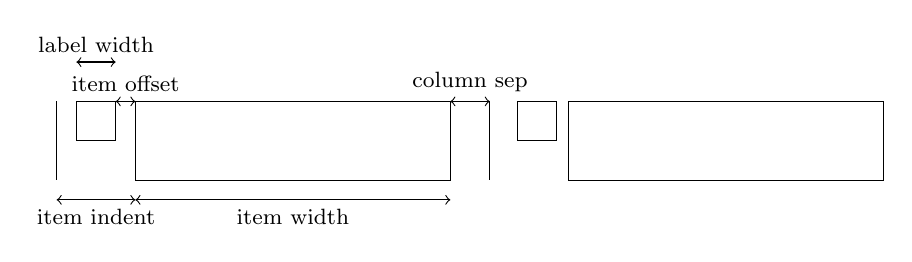
\begin{tikzpicture}[every node/.style={font=\footnotesize},scale=.5]
    \coordinate (itemedge1) at (2,2) ;
    \coordinate (itemedge2) at (13,2) ;
    \draw
      (itemedge1) -- ++(8,0) -- ++(0,-2) -- ++(-8,0) -- cycle ;
    \draw
      (itemedge1) ++(-.5,0) coordinate(labeledge1)
      -- ++(-1,0) --++ (0,-1) --++(1,0) --++(0,1) ;
    \draw (itemedge1) ++(-2,0) -- ++(0,-2) ;
    \draw
      (itemedge2) -- ++(8,0) -- ++(0,-2) -- ++(-8,0) -- cycle ;
    \draw
      (itemedge2) ++(-.3,0) coordinate(labeledge2)
      -- ++(-1,0) --++ (0,-1) --++(1,0) --++(0,1) ;
    \draw (itemedge2) ++(-2,0) -- ++(0,-2) ;
    \draw[<->] (itemedge2) ++(-2,0) --node[above]{column sep} ++(-1,0) ;
    \draw[<->] (0,-.5) --node[below]{item indent} (2,-.5) ;
    \draw[<->] (2,-.5) --node[below]{item width} (10,-.5) ;
    \draw[<->] (labeledge1) ++(0,1) --node[above]{label width} ++(-1,0) ;
    \draw[<->] (labeledge1) --node[above]{item offset} ++(.5,0) ;
  \end{tikzpicture}
  \caption{A visual representation of the used lengths.}
  \label{fig:lengths}
\end{figure}

Now the same list as above but with three columns and a different label:
\begin{example}
  \begin{tasks}[counter-format=(tsk[r]),label-width=4ex](2)
    \task \Sample
    \task \sample\ \sample
    \task \sample
    \task \Sample
    \task \sample\par\sample
  \end{tasks}
\end{example}
% \begin{tasks}[counter-format=(tsk[r]),label-width=4ex](3)
%  \task \Sample
%  \task \sample\ \sample
%  \task \sample
%  \task \Sample
%  \task \sample\par\sample
% \end{tasks}

Let's use it inside a question, \ie, inside \ExSheets' \env{question}
environment:
\begin{example}
  % since settings are local the following ones will be lost
  % outside this example;
  \settasks{
    counter-format = qu.tsk ,
    item-indent    = 2em ,
    label-width    = 2em ,
    label-offset   = 0pt
  }
  \begin{question}[type=exam]{4}
    I have these two tasks for you. Shall we begin?
    \begin{tasks}(2)
      \task The first task: easy!
      \task The second task: even more so!
    \end{tasks}
  \end{question}
  \begin{solution}[print]
    Now, let's see\ldots\ ah, yes:
    \begin{tasks}
      \task This is the first solution. Told you it was easy.
      \task This is the second solution. And of course you knew that!
    \end{tasks}
  \end{solution}
\end{example}

Finally let's see what the \option{debug} option does (you could see it
already on page~\pageref{debug}):
\begin{example}
  \settasks{debug}
  \begin{tasks}(2)
    \task \Sample
    \task \Sample
  \end{tasks}
\end{example}

\section{Available Instances}\label{sec:tasks:instances}
When you use the package option \option{more} of the \Tasks\ package or load
\ExSheets\ with the \option{load-tasks} option there are currently three
additional instances for the \code{tasks} object available:
\begin{description}
  \item[itemize] uses \cs*{labelitemi} as labels.
  \item[enumerate] enumerates the items with 1., 2., \ldots
  \item[multiplechoice] a --~well~-- `multiple choice' list.
\end{description}
\begin{example}
  \begin{tasks}[style=itemize](2)
    \task that's just how\ldots
    \task \ldots we expected
  \end{tasks}
  \begin{tasks}[style=enumerate](2)
    \task that's just how\ldots
    \task \ldots we expected
  \end{tasks}
  \begin{tasks}[style=multiplechoice](2)
    \task that's just how\ldots
    \task \ldots we expected
  \end{tasks}
\end{example}

\section{Custom Labels}
If you want to change a single label inside a list, you can use the optional
argument of \cs{task}. This will temporarily overwrite the default label.
\begin{example}[side-by-side]
  \begin{tasks}[style=itemize]
    \task a standard item
    \task another one
    \task[+] a different one
    \task and another one
  \end{tasks}
\end{example}

\section{New Tasks}
It is possible to add custom environments that work like the \code{tasks}
environment.
\begin{commands}
  \command{NewTasks}[\oarg{options}\marg{name}\oarg{separator}\darg{cols}]
    Define environment \meta{name} that uses \meta{separator} to introduce a
    new item.  Default for \meta{separator} is \cs{task}, default for
    \meta{cols} is \code{1}.  The \meta{options} are the ones described in
    section~\ref{sec:tasks:options}.
  \command{RenewTasks}[\oarg{options}\marg{name}\oarg{separator}\darg{cols}]
    Renew environment previously defined with \cs{NewTasks}.
\end{commands}
The \env{tasks} environment is defined as follows:
\begin{sourcecode}
  \NewTasks{tasks}
\end{sourcecode}

The separator does not have to be a control sequence:
\begin{example}
  % preamble:
  % \usepackage{dingbat}
  \NewTasks[label=\footnotesize\leftthumbsup,label-width=1.3em]{done}[*]
  \begin{done}
    * First task
    * Second task
  \end{done}
\end{example}
Although this might seem handy or even nice I strongly advice against using
something different than a command sequence. Remember that the items will be
split at \emph{every} occurrence of the separator.  So in order to use the
separator (here for example for a starred variant of a command) within an item
it has to be hidden in braces.  This is avoided of you use a command sequence
which even doesn't have to be defined.

Please also keep in mind that the separator still has an optional star
argument (see~\pageref{optional-star}), an optional bang argument and the
standard optional argument.  Using \code{*} will prevent the optional star
argument.

\begin{example}
  % preamble:
  % \usepackage{dingbat}
  \NewTasks[label=\footnotesize\leftthumbsup,label-width=1.3em]{done}[*]
  \begin{done}(3)
    * First task
    * Second task
    *! Third task spanning the full width available
    * Fourth task
  \end{done}
\end{example}

Let's say you want a \env*{multiplechoice} environment that has three columns
in its default state.  You could do something like this:
\begin{example}
  % preamble:
  % \NewTasks[style=multiplechoice]{multiplechoice}[\choice](3)
  % \newcommand*\correct{\PrintSolutionsTF{\checkedchoicebox}{\choicebox}}
  %
  % \PrintSolutionsTF and the {question} environment are provided
  % by the ExSheets package
  \begin{question}
    \begin{multiplechoice}
      \choice First choice
      \choice Second choice
      \choice[\correct] Third choice
    \end{multiplechoice}
  \end{question}
  \begin{solution}[print]
    \begin{multiplechoice}
      \choice First choice
      \choice Second choice
      \choice[\correct] Third choice
    \end{multiplechoice}
  \end{solution}
\end{example}

The last example shows you two additional commands:
\begin{commands}
  \command{choicebox}[\quad\choicebox]
    Print an empty square.
  \command{checkedchoicebox}[\quad\checkedchoicebox]
    Print a crossed-out square.
\end{commands}


\section{Styling \Tasks}
Equivalent to the styling of \ExSheets\ \Tasks\ uses \pkg{xtemplate} to
declare additional instances for the lists.

\subsection{The \code{tasks} Object}\label{sec:tasks}
The object that's defined by \Tasks\ is the `tasks' object.  This time there
are four instances available for the one template (again `default') that was
defined.

\subsubsection{Available Options}
This section only lists the options that can be used when defining an instance
of the `default' template.  The following subsections will give some examples
of their usage.

\begin{sourcecode}
  \DeclareTemplateInterface{tasks}{default}{3}
    {
      % option        : type      = default
      enumerate       : boolean   = true    ,
      label           : tokenlist           ,
      indent          : length    = 2.5em   ,
      counter-format  : tokenlist = tsk[a]) ,
      label-format    : tokenlist           ,
      label-width     : length    = 1em     ,
      label-offset    : length    = .3333em ,
      after-item-skip : skip      = 1ex plus 1ex minus 1ex
    }
\end{sourcecode}

\subsubsection{Predefined Instances}
This is rather brief this time:
\begin{sourcecode}
  % ALPHABETIZE: a) b) c)
  \DeclareInstance{tasks}{alphabetize}{default}{}
  % available when `load-tasks=true':
  % ITEMIZE:
  \DeclareInstance{tasks}{itemize}{default}
    {
      enumerate   = false ,
      label-width = 1.125em
    }
  % ENUMERATE:
  \DeclareInstance{tasks}{enumerate}{default}
    { counter-format = tsk. }
  % MULTIPLECHOICE:
  \DeclareInstance{tasks}{multiplechoice}{default}
    {
      enumerate = false       ,
      label     = \choicebox  ,
    }
\end{sourcecode}

\end{document}
